\chapter{Implementierung}

\begin{figure}[ftb]
\label{HauptAblauf}
\centering
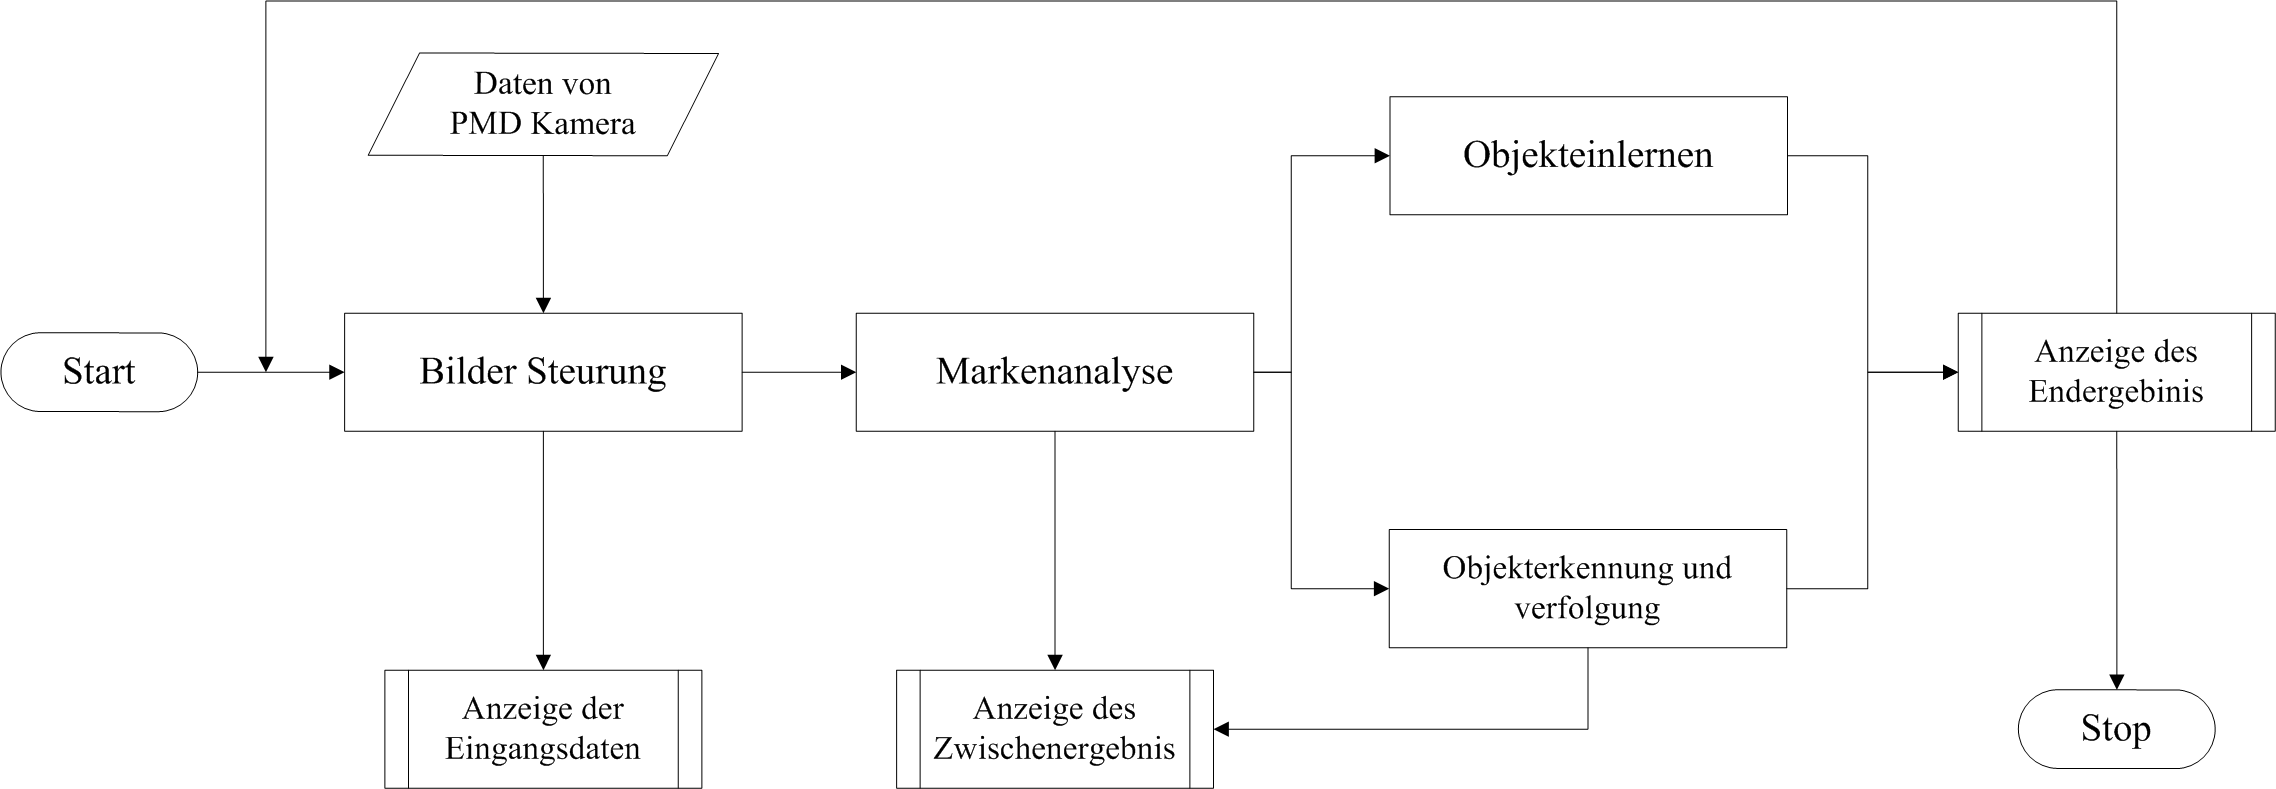
\includegraphics[scale=0.55]{Abbildungen/HauptAblauf.png}
\caption{Ablaufdiagramm}
\end{figure}

Unsere Implementierung kann in 4 Hauptmodule unterteilt werden:

\begin{itemize}
\item Markenanalyse
\item Objekteinlernen
\item Objekterkennung und Verfolgung
\item Bilder Steuerung
\end{itemize}

Die allgemeine Ablaufprozess des Programms findet man in Abbildung~\ref{HauptAblauf}. Das ganz Programm ist eine Schleife. In jedem Schritt wird die Information von PMD Kamera angesammelt und als Eingabe eingegeben. Nach Bewertung der neuen Eingabe bzw. der R�ckkopplung von letztem Ablauf wird die entsprechende Bilddaten von Modul Bilder Steuerung f�r die weiteren Schritten ausgew�hlt. Der Modul Markenanalyse analysiert die eingegebene Bilddaten und versucht die Marken zu finden und zu verfolgen. Die ausgefundene Marken werden von entweder dem Objekteinlernen oder der Objekterkennung und Verfolgen benutzt, welche am Anfang des Programms durch Benutzer entschieden wird. In der Einlernensphase wird zuerst die Transformation des Objekts bestimmt und dann das charakteristische Graph des Objekts durch die Marken dargestellt. Wenn man ein Objekt wieder erkennen m�chte, werden die Marken von neuem Objekt zu den vorhandenen charakteristischen Graphen verglichen, die nach dem Objekteinlernen im Speicher gespeichert werden. Das Ergebnis wird in einem OpenGL Fenster ausgemalt und au�erdem,  als die R�ckkopplung f�r den n�chsten Schritt zur�ck zum Anfang der Schleife geschickt. Alle diese Module werden in folgenden Unterabschnitten genau erkl�ren und ein ausf�hrliches Ablaufdiagramm wird in Abbildung~\ref{GenauAblauf} gezeigt.   

\begin{figure}
\label{GenauAblauf}
\centering
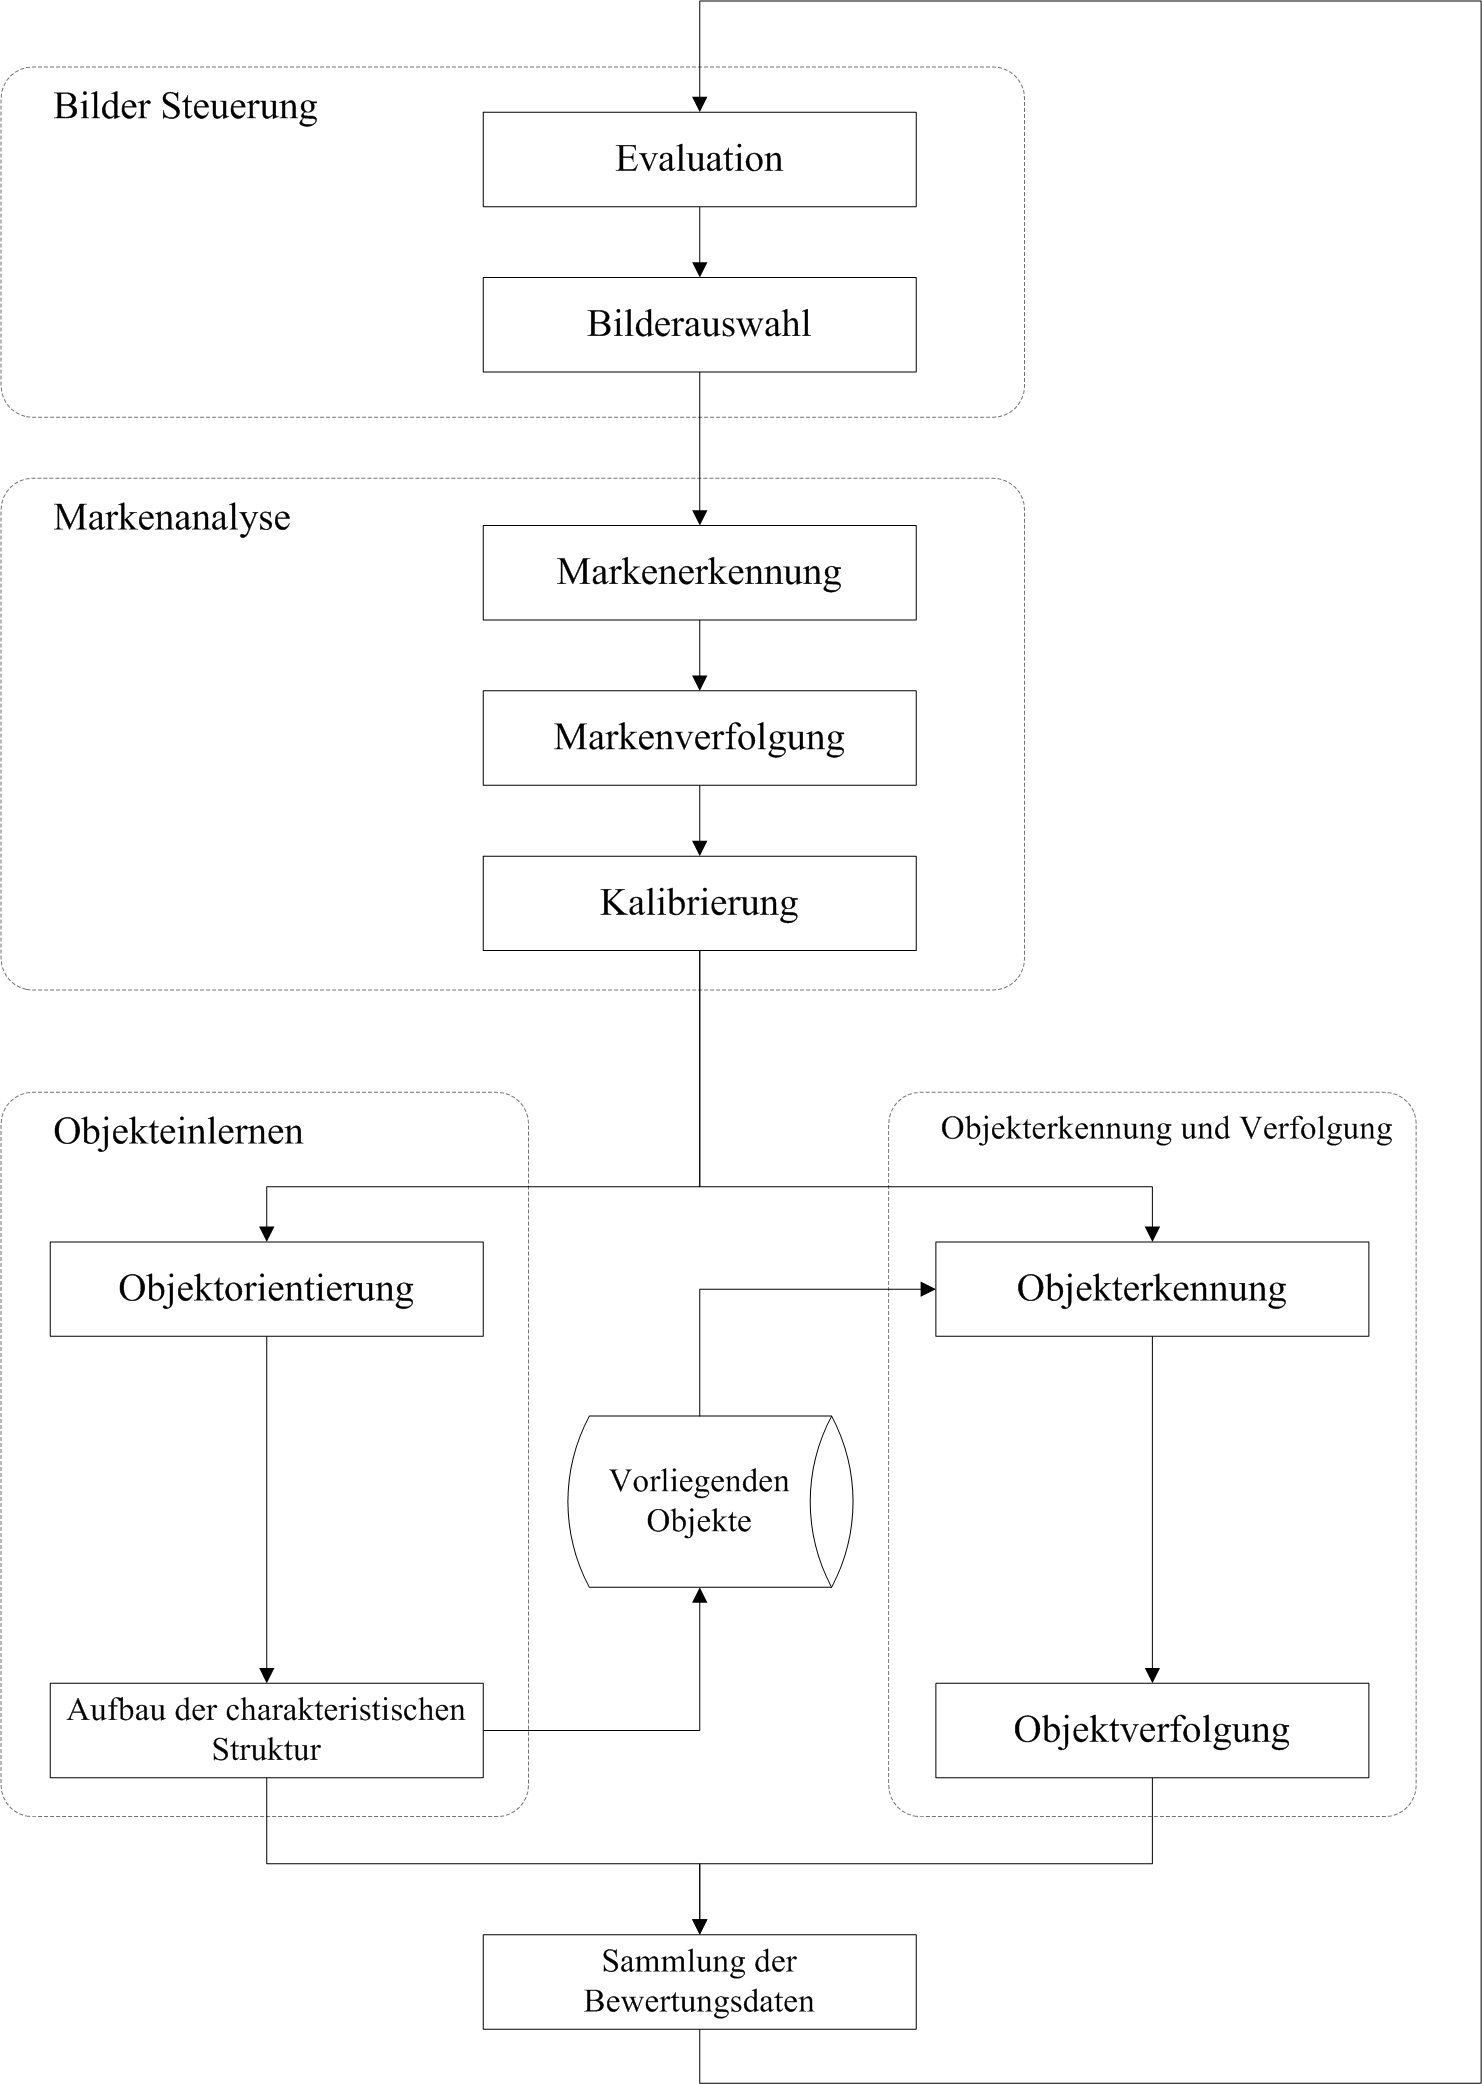
\includegraphics[scale=0.7]{Abbildungen/Ablaufsbild.png}
\caption{Ausf�hrliches Ablaufdiagramm}
\end{figure}

\section{Markenanalyse}

\subsection{Markenerkennung}

\subsubsection{Auswahl der Gr��e der Marken}
Die Erkennungsergebnisse der Objekte werden von der Gr��e der Marken stark beeinflusst, deshalb ein Test �ber die Markengr��e zuerst notwendig ist. Die Testmarken werden in wei�e auf einem schwarzen Papier gedruckt. Es gibt insgesamt 7 verschiedenen Gro�stufen, und die Marken von jeder Stufe werden durch jeweils Quadrat und Kreis formuliert. Abbildung~\ref{MS1} zeigt die unterschiedliche Erkennungsergebnisse der Marken, wenn das Objekt am verschiedenen Positionen aber auf der gleichen Ebene liegt. Abbildung~\ref{MS2} zeigt den Einfluss auf den Ergebnisse von der Distanz zu der Kamera. Was deutlich ist, dass je n�her das Objekt von der Kamera angebracht wird, desto kleinere die Gr��e der Marken ben�tigt.

\begin{figure}
\centering
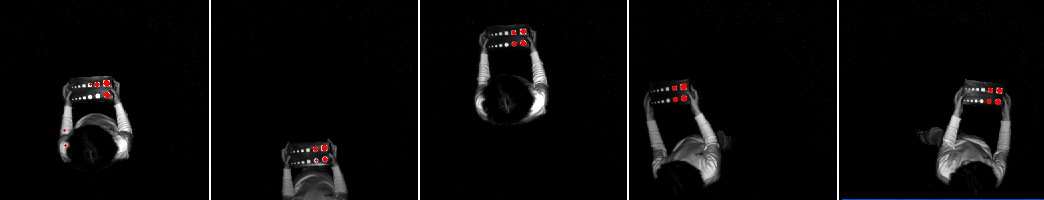
\includegraphics[scale=0.5]{Abbildungen/MarkerSize1.png}
\caption{Die Erkennungsergebnisse der Marken f�r unterschiedliche Positionen.}
\label{MS1}
\end{figure}

\begin{figure}
\centering
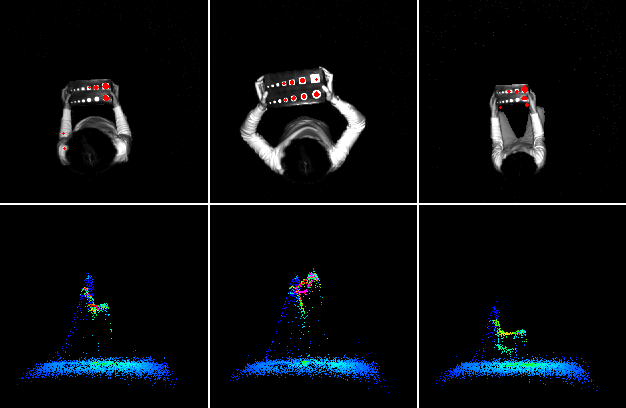
\includegraphics[scale=0.9]{Abbildungen/MarkerSize2.png}
\caption{Die Erkennungsergebnisse der Marken f�r unterschiedliche Distanz zu der Kamera. Auf der ersten Reihe liegen die Graustufenbilder mit roten erkannten Marken; Die entsprechende 3D Bilder auf der zweiten Reihe zeigen die vertikalen Positionen des Objekts.}
\label{MS2}
\end{figure}

\subsubsection{Kontrolle der Helligkeit}

\subsection{Markenverfolgung}

\section{Objekteinlernen}

\subsection{Markenanordnung}

\subsection{Kanteneinf�gung}

\subsection{Speichern des Strukturgraph}

\section{Objekterkennung und Verfolgung}

\subsection{Vergleichung der Objekte}

\subsection{Bestimmung der Orientierung}

\section{Bilder Steuerung}